\section{Experimental data and experimental method}

\subsection{ALICE}
\subsubsection{Overview}
\begin{itemize}
    \item Trigger System
    \item ITS
    \item TPC % discuss boethe bloch in detail here
    \item TOF
	\item V0
\end{itemize}

\subsubsection{Basics of ALICE data structure}
ALICE data is split by runs, then by events, and within the event by tracks, as is shown in figure \ref{fig:ALICE_data_schematic}. Runs are periods of time during which collisions with the same conditions occurred, which means that the data taking is started and kept up until there is some problem which requires the run to be ended. This means that runs are of arbitrary length. They are denoted by LHC + the last two digits of the year in which the data was taken + a letter of the alphabeth, sequentially used, e.g.: LHC17a is the first data run taken during 2017. Once the raw data is taken, the Data Preparation Group (DPG) is responsible for doing a reconstruction pass over the data, which means to build the tracks from the individual detector hits, correcting for any calibration or distortion effects. The data structure  one is left with is a list of events, each of which contain a list of tracks. This is what is subsequently used by analysers. 

\begin{figure}
	\includegraphics[]{}
	\centering
	\caption{Schematic of the data structures within ALICE. The data is split by run periods, then by event, and within the event by tracks. }
		\label{fig:ALICE_data_schematic}
\end{figure}
\subsubsection{Collision system and event cuts}
The data provided in ALICE by necessity includes a large range of particles and impurities, since for each analysis what qualifies as impurities changes. Therefore, cuts are applied at the analysis level, to provide a much cleaner environment for the actual analysis. Within the analysis, these cuts happen on both an event and a track level, leaving a subset of tracks which can be analyzed. The goals of these cuts are: i) to cut bad quality tracks, where the PID is not certain, ii) to cut tracks of uninteresting particles for the specific analysis, e.g. weak decays in the analyses in this thesis and iii) to reduce the background, such as from secondary particles. These cuts also vary between collision systems, which is necessitated by their different properties. To exemplify, lets compare high multiplicity pp and Pb--Pb collisions. In HM pp collisions the mean multiplicity is 34, while in central lead lead collisions it is about 1000. This means that the mean occupancy of the detectors is much greater in Pb--Pb collisions, which in turn means that the tracking algorythm has a higher chance to assign a wrong cluster to a track. In order to reduce this effect, the matching window for the TOF detector is reduced in Pb--Pb collisions, from 10 cm to 3 cm. For the analysis method explained in section \ref{sec:TOFTPC}, this introduces an uncertainty, as some tracks could be elastically scattered in the TRD or space frame, causing them to miss the matching window without having interacted inelastically. This would mean that there is an elastic contribution to the inelastic cross section meassured using the TOF/TPC method. To evaluate and counteract this, a special reconstruction of the Pb--Pb data was done for the Pb--Pb results shown in this thesis, where the matching window was set to 10 cm instead of 3 cm. The effect of this change is explained in section \ref{sec:TOFTPC}. \\

The main selection criteria for the event was its multiplicty. The multiplicity measures the number of charged particles at mid-rapidity, and for this analysis the top 0-0.17\% of high multiplicity pp events were used. This data is selected by a trigger, called the high multiplicity trigger (using the kHighMult flag in the ALICE analysis framework), which triggers on the V0 multiplicity measurement. HOW ARE THESE RELATED? 

\subsubsection{Reconstruction of raw (anti)nuclei spectra}
In order to obtain the raw antinuclei spectra, the tracks first have to be identified as antinuclei. This particle identification (PID) occurs on the basis of two main detectors: the TPC and the TOF. Due to the distinct masses of antinuclei (they are heavier than most other long lived particles), they leave a distinct signal in each detector. In the TPC, antideuterons are clearly seperated by their energy loss up to a momentum of about 1.4 GeV. For antitriton, the seperation works until a momentum of 1.X GeV. \ahe\ is well sepatared from lighter particles in the TPC for all momenta, due to its double charge. Since the energy loss rises with $Z^2$, the energy loss of \ahe\ is characteristically much higher than those of singly charged particles. \\
In the TOF, the time of flight measurement combined with the track length and curvature gives a measurement of the particles mass, according to equation \ref{eq:TOFm2}. This allows a clean signal for antitriton and \ahe\. For antideuterons, there is still a significant contamination from the tail of the proton distribution at those masses, which requires a fit to the signal and the background to extract the antideuteron yield. Figures \ref{fig:TPC_fits_ahe} and \ref{fig:TOF_fits_ahe}, \ref{fig:TPC_fits_trit} and \ref{fig:TOF_fits_trit}, show the extraction procedure in the TPC and TOF, for \ahe\ and \atrit\, respectively. The particle and antiparticle distributions are fit with a gaussian function. For \ahe\ , a second gaussian is used to account for the background from (anti)triton. Their respective signals in the TOF detector are very clean, as is shown in figures \ref{fig:TOF_fits_ahe} and \ref{fig:TOF_fits_trit}, therefore, the TOF signal is used by applying a cut on the $m_{TOF}^2$. An example figure of the antideuteron extraction in the TOF is shown in figure \ref{fig:dbar_TOF_fit}(for more details see \cite{dbar_ann}). The combination of these measurement allows the extraction of the (anti)nuclei spectra, which are shown in \ref{fig:(anti)nucleiSpectra}. The combined signal extraction cuts are shown in table \ref{tab:PIDcuts}.

\begin{equation}\label{eq:TOFm2}
    
\end{equation}

\begin{table}
%todo insert table of PID cuts from analysis notes.
\end{table}

%todo: insert all the PID figures from the he3bar and atrit analyses.
%todo: write a paragraph and insert figures on different fitting algorythms in AliPhysics, what they do and how this affects low statistics analyses -> i.e. a lot. Also talk about errors on the 0 bins here. 
\subsubsection{Raw \ratio\ \ and antitriton-to-triton ratio}
\subsubsection{Correction for secondaries from material spallation}
In order to obtain pure samples of nuclei, any secondary nuclei not created need to be subtracted from the obtained raw spectrum. Two sources of secondary particles exists: weak decays and material spallation. For \ahe\ and \atrit\, weak decays are negligible, since the amount of $^3H_\Lambda$ measured in pp collisions is xx the amount of \ahe\, as can be seen from figure \ref{}. The branching ratio of $^3H_\Lambda \rightarrow $ \ahe\ is expected to be 25\% \cite{PDG}. Thus, secondary nulcei from material spallation remain, which shall simply be referred to as secondaries hereinafter. Since these secondaries are created by essentially "knocking out" these nuclei from larger nuclei in the ALICE detector material and in the beampipe, no secondary antinuclei exist. In order to differentiate between secondaries and primaries, we make use of the fact that all primaries have a common origin (called the primary vertex), while the distribution of secondaries should not point to the primary vertex. The measure of how close a particle's track reaches to the primary vertex is known as the distance of closest approach (DCA), and within ALICE is resolved in both the $xy$ and the $z$ planes. So, from physical expectations we expect the primary DCA distribution to be peaked sharply at 0, while the distributions for secondaries should be mainly flat. Example distributions from Monte Carlo Simulations are shown in figure \ref{fig:}.


%todo include figure for hypertriton to he3 ratio
%todo include figure for exemplary DCA distributions 
Figure \ref{fig:} shows that while the distribution for primaries is indeed sharply peaked at 0, the distribution of secondaries is not flat, but also peaks around 0. This is an experimental effect due to the tracking algorithm, which prefers reconstructing tracks pointing towards the primary vertex. This is excacerbated by the possibility to assign a wrong ITS cluster to the track. Several cuts can be made on the tracks to minimize this effect, which are outlined in section \ref{sec:event and track selection}. The most important cut is on the number of clusters in the first ITS layer, which reduces the number of secondary tracks by XX\%, as is shown in figure \ref{fig:thatone->} %todo insert figure here showing the distributions before and after this cut.
\\
In order to extract the secondary fraction from the DCA distributions, template fits are used. These fits take the shape of input templates (in this case from primaries and from secondaries) and try to match their relative contribution in order to reproduce the shape in data. Two different fitting algorithms exists for this purpose within the ALICE analysis framework: the TFractionFitter and Roofit. The main difference between the two is that the TFractionFitter can change the shape of the templates within uncertainties in order to better reproduce the data. In the limit of infinite statistics, both of these methods should produce the same result. In the analyses shown in this thesis, the TFractionFitter was used as the default method, and Roofit was used to crosscheck these results. \\
The biggest challenge with secondary corrections is to get reliable templates for secondary nuclei from material. For a combinatorial background, a side band analysis can be done, since no deviating behaviour in the signal region is expected, but since we have already seen in figure \ref{} that secondary tracks are also peaked towards the primary vertex, the sideband analysis cannot help us account for this. It is however also impossible to extract a pure secondary distribution from data, since the peak region always necessarily includes the particles produced in the initial collision. Thus, we need to simulate the distribution with Monte Carlo simulations. This means that we rely on the assumption that all the involved processes are accurately reproduced in Monte Carlo, specifically, we rely on the fact that the angular distribution of the spallation processes are accurately reproduced\footnote{The absolute value of the cross section is not important for the accuracy of the templates, since the relative weight is later determined by the template fits. However, too low a cross section means that far more events have to be simulated in order to gain sufficient statistics to obtain the template.}. The advantage of this method, is that in full ALICE Monte Carlo simulations, the same tracking algorithm is used as in data reconstruction, which means that if the spallation processes are accurately simulated, the distribution will match the true distribution. Also, these simulations rely on the correct underlying event, i.e. for high multiplicity pp collisions, such collisions need to be accurately simulated. This is due to the fact that the spallation is triggered by particles produced in the primary collision. A final challenge to obtaining the template fits is the rarity of these spallation processes in MC simulations. 

%write about rarity of these processes, back it up with the general purpose calculations, write for the need for the special reconstruction, and compare Geant3/Geant4 distributions

\\ \\ \\ 

One could also ask the question of which primary particles are responsible for the largest amounts of nuclei secondaries from spallation. In order to investigate this question, a toy Monte Carlo simulation was used, where beams of primary particles were fired on layers of beryllium and beryllium + carbon, corresponding to the materials of the beampipe and the support structure of the first ITS layers. This configuration was chosen since if the spallation occurs later, the missing hit in the first ITS layer allows a large degree of rejection\footnote{This is somewhat less true in Pb-Pb collisions, since the multiplicities are so much higher and therefore a wrongly associated ITS cluster is far more likely.}. An exponential energy spectrum was used for the primary particles, tuned to the proton spectrum measured by ALICE \cite{}. Geant4 was employed for this simulation. The resulting yields of secondary deuterons and $^3\mathrm{He}$ are shown in figure \ref{fig:toyMCGeant4Spallation}. Interestingly, the primary antiparticles produce a larger portion of the secondary nuclei than their particle partners. Also, while antideuterons produce a larger amount of secondary nuclei than antiprotons (by roughly 2x), given that their relative abundance in pp collisions is 1000x less, their contribution is expected to be on the sub \% level. This leads to the conclusion that it is mainly (anti)protons and pions which are responsible for creating secondary antinuclei. Therefore, when using ALICE Monte Carlo simulations, it is not necessary to employ a coalescence afterburner with the underlying event in order to accurately simulate the secondary distributions. A caveat to this is that the simple toy Monte Carlo simulation only probed absolute yields, rather than the angular distribution, and as already noted above, the latter is the important factor. However, given that the contribution to the yields is on the sub \% level, any difference in the distribution is expected to be negligible. 

\begin{figure}[hbtp]
    \centering
    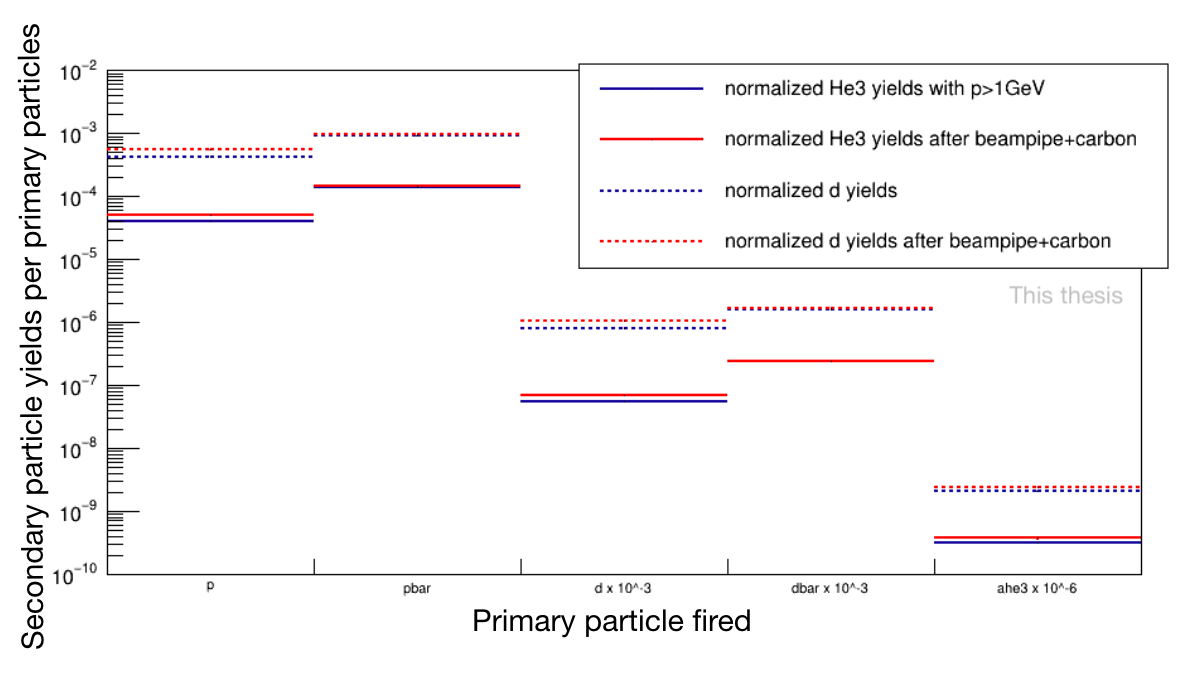
\includegraphics[width=\textwidth]{figures/simpleMC_secondaries_G4.png}
    \caption{Results of a simple toy Monte Carlo simulation of a particle beam on materials mimicking the LHC beampipe in ALICE and the beampipe + ITS support structure. The resulting secondary deuterons and $^3\mathrm{He}$ are shown as a function of the primary particle fired, where the results are roughly scaled by the primary particles relative abundance.}
    \label{fig:toyMCGeant4Spallation}
\end{figure}
\subsubsection{Annihilations within the detector}
Annihilations within the detector material can occur at any point within the detector, but are of course more likely in denser materials. For the purpose of this discussion we shall differentiate between 3 different scenarios: i) annihilations before the middle of the TPC, since such tracks cannot be identified and will therefore not be reconstructed in our spectra. ii) annihilations between the middle of the TPC and the TOF, since these annihilations can be directly probed by the comparison of the yields in the TPC and TOF. And finally annihilations outside of the TOF detector, which for the purposes of this analysis is not seen at all, i.e. such annihilations are not measured. \\

Let us first consider the case where the annihilation occurs before the middle of the TPC. A track with less than half of the TPC clusters will be removed by the track cuts, therefore this track will not show up in our analysis. 


\subsection{Extracting the inelastic cross section from the antimatter-to-matter ratio}
The idea behind using the antimatter-to-matter ratio as the observable to measure the antinuclei inelastic cross section, is that antinuclei will annihilate in the detector material, and therefore disappear from our measurement. In order to quantify the inelastic cross section we thus need to know how many particles were originally produced, i.e. we need to normalise the antinuclei spectrum to the number of originally produced antinuclei. However, we cannot use theoretical predictions tuned to this data, since that would be a circular argument, i.e. we would get out the same inelastic cross section as we put in. Therefore, the matter nuclei are used as a proxy instead. This works very well for a few reasons. First, the matter inelastic cross section can be easily measured, and have been measured for deuterons \cite{}, helium-3\cite{} and tritons\cite{}. Second, other effects affecting acceptance or efficiency will largely cancel between the nuclei and antinuclei counterparts, since the two only differ in their charge sign. Third and perhaps most important, is the fact that at LHC energies, the baryochemical potential is very close to 0, and has been accurately measured for antiprotons. This means that we know to a very high degree of accuracy how many antinuclei are produced relative to the produced nuclei, and the other processes by which both might be lost within the detector are also well understood. Thus, the antimatter-to-matter ratio is sensitive to the antinuclei inelastic cross section, and other variables it is sensitive to are well understood and under control. This makes this ratio such a promising probe to measure the inelastic cross section.\\

Having established that the antimatter-to-matter ratio is sensitive to the inelastic cross section, it is still not trivial to extract the inelastic cross section from this observable. This difficulty is due to having to account for many processes. One example is the path which the particles take through the detector. In the magnetic field, (anti)nuclei travel on curved tracks, so the amount of matter they interact with will depend on their initial trajectory. This thus needs to be averaged over the $\eta$ distribution of the antinuclei. This is just one of many similar effects which make an analytical relationship between the antimatter-to-matter ratio and the antinuclei inelastic cross section difficult to achieve. Thankfully, there is a superior option with detailed Monte Carlo simulations. Detailed simulations of the ALICE detector using Geant4 account for such processes, and by changing the inelastic cross section in these simulations, we can probe its relationship to the antinuclei-to-nuclei ratio.
\subsubsection{Comparison of ratios with Monte Carlo simulations}\label{sec:MCSim}
In order to fairly compare the Monte Carlo simulations to the produced data, it is vital to account for the baryochemical potential\footnote{In other words: how much more antimatter particles we have for each matter particle. Given that we collide purely matter particles, there is a penalty for producing antimatter, even though at such high energies it is vanishingly small.} at such high energies. The relevant ratio of antiprotons to protons is shown in figure \ref{fig:BaryochemicalPotential}. Based on the same arguments as the formula for the coalescence parameter \ref{eq:CoalescenceParameter}, the effect on the ratio of antinuclei will be the same as to the antiproton-to-proton ratio taken to the exponent of the mass number of the antinucleus. 

\begin{figure}
    \centering
    \includegraphics{}
    \caption{Ratio of antiprotons to protons produced at mid-rapidity as a function of beam rapidity. At ALICE energies the value approaches unity, demonstrating that at such high energies antimatter and matter are produced in almost equal amounts.}
    \label{fig:BaryochemicalPotential}
\end{figure}
\subsubsection{Ratios as a function of the inelastic cross section}
\subsubsection{Non-linear error propagation}
\subsubsection{Accounting for energy losses between the primary vertex and the point of annihilation}
\subsubsection{Uncertainty coming from the material budget}
\subsubsection{Evaluating the average material for antinuclei annihilations in the ALICE detector}
\subsubsection{Independence of collision system}
The antimatter-to-matter ratio method's dependence on collision system has been investigated by redoing the analysis performed in pPb collisions in \cite{dbarIvan} for high multiplicity pp collisions. The dependence on the collision system is due to the multiplicity differences, and the resulting difference in the baryochemical potential as discussed in section \ref{sec:MCSim}. By taking the antiproton-to-proton ratio for the different collision systems and comparing them, the predicted difference between the antideuteron-to-deuteron ratio was obtained. The results are shown in figure \ref{fig:pp_pPb_dbardRatio}, which show that the differences between collisions systems are consistent with the expected deviation. This independence of the collision system is expected, since the inelastic cross section is completely independent on the collision system. This becomes especially self-evident when considering that the annihilations do not occur in the initial collisions, but rather as the antiparticles travel through the detector material.

\begin{figure}[h]
    \centering
    \includegraphics{}
    \includegraphics{}
    \caption{Ratio of the antiproton-to-proton ratios (left) and antideuteron-to-deuteron ratios (right) obtained in high multiplicity pp collisions and in pPb collisions, compared to the expected difference from the different baryochemical potentials (dashed red line).}
    \label{fig:pp_pPb_dbardRatio}
\end{figure}

